% questions.tex —— 2017 年·全国Ⅲ卷·理科 · 题目内容片段（无答案）
% 由 tools/generate_projects.py 依来源总账自 2017/2017_数学真题_全国3理_试题.md 生成，勿手改（改源 MD 后重跑）


\gkpart{数学}

\begin{gktip}
\textbf{来源说明}：本题面依据固定源 PDF 两页 A3 页面逐题核对，原卷印刷页码 1045–1046。固定源不附答案；本文件仅为题面规范源。
\end{gktip}

\gkpart{一、选择题}

\begin{question}
\gkti{1}已知集合 \(A=\{(x,y)\mid x^2+y^2=1\}\)，\(B=\{(x,y)\mid y=x\}\)，则 \(A\cap B\) 中元素的个数为（　）

   （A）3　　（B）2　　（C）1　　（D）0

\end{question}
\begin{question}
\gkti{2}设复数 \(z\) 满足 \((1+i)z=2i\)，则 \(|z|=\)（　）

   （A）\(\dfrac12\)　　（B）\(\dfrac{\sqrt2}{2}\)　　（C）\(\sqrt2\)　　（D）2

\Needspace{0.4\textheight}
\end{question}
\begin{question}
\gkti{3}某城市为了解游客人数的变化规律，提高旅游服务质量，收集并整理了 2014 年 1 月至 2016 年 12 月期间月接待游客量（单位：万人）的数据，绘制了下面的折线图。
\nopagebreak[4]
\begin{center}\begin{tikzpicture}[x=0.28cm,y=0.25cm,line cap=round,line join=round,font=\scriptsize]
\draw[->] (0,0)--(37,0);
\draw[->] (0,0)--(0,21);
\foreach \y/\lab in {0/25,5/30,10/35,15/40,20/45} {
  \draw[densely dashed,gray!65] (0,\y)--(36.5,\y);
  \node[left] at (0,\y) {\lab};
}
\foreach \x in {1,...,36} {
  \draw (\x,0)--(\x,-0.35);
  \pgfmathtruncatemacro{\month}{mod(\x-1,12)+1}
  \node[below] at (\x,-0.55) {\month};
}
\draw[thick] plot[mark=*,mark size=0.65pt] coordinates {
  (1,1.5)(2,2.5)(3,2)(4,4)(5,3.5)(6,3)(7,8)(8,10)(9,5.5)(10,7)(11,4.5)(12,3.5)
  (13,6)(14,6.5)(15,5.5)(16,7)(17,7)(18,6)(19,11)(20,12.5)(21,8.5)(22,10)(23,7.5)(24,7)
  (25,7.5)(26,8)(27,10)(28,11.5)(29,11)(30,10)(31,9)(32,14.5)(33,17)(34,12)(35,14)(36,10)
};
\draw (0.1,-0.15)--(-0.1,0.05)--(0.1,0.25);
\node[left] at (-0.25,-0.85) {$O$};
\node at (18,22.4) {月接待游客量（万人）};
\node at (6.5,-2.2) {2014 年};
\node at (18.5,-2.2) {2015 年};
\node at (30.5,-2.2) {2016 年};
\end{tikzpicture}
\end{center}
\nopagebreak[4]
   根据该折线图，下列结论错误的是（　）

   （A）月接待游客量逐月增加

   （B）年接待游客量逐年增加

   （C）各年的月接待游客量高峰期大致在 7、8 月

   （D）各年 1 月至 6 月的月接待游客量相对于 7 月至 12 月，波动性更小，变化比较平稳

\end{question}
\begin{question}
\gkti{4}\((x+y)(2x-y)^5\) 的展开式中的 \(x^3y^3\) 系数为（　）

   （A）\(-80\)　　（B）\(-40\)　　（C）40　　（D）80

\end{question}
\begin{question}
\gkti{5}已知双曲线 \(C:\dfrac{x^2}{a^2}-\dfrac{y^2}{b^2}=1\ (a>0,b>0)\) 的一条渐近线方程为 \(y=\dfrac{\sqrt5}{2}x\)，且与椭圆 \(\dfrac{x^2}{12}+\dfrac{y^2}{3}=1\) 有公共焦点，则 \(C\) 的方程为（　）

   （A）\(\dfrac{x^2}{8}-\dfrac{y^2}{10}=1\)　　（B）\(\dfrac{x^2}{4}-\dfrac{y^2}{5}=1\)　　（C）\(\dfrac{x^2}{5}-\dfrac{y^2}{4}=1\)　　（D）\(\dfrac{x^2}{4}-\dfrac{y^2}{3}=1\)

\end{question}
\begin{question}
\gkti{6}设函数 \(f(x)=\cos\left(x+\dfrac\pi3\right)\)，则下列结论错误的是（　）

   （A）\(f(x)\) 的一个周期为 \(-2\pi\)

   （B）\(y=f(x)\) 的图象关于直线 \(x=\dfrac{8\pi}{3}\) 对称

   （C）\(f(x+\pi)\) 的一个零点为 \(x=\dfrac\pi6\)

   （D）\(f(x)\) 在 \(\left(\dfrac\pi2,\pi\right)\) 单调递减

\Needspace{0.4\textheight}
\end{question}
\begin{question}
\gkti{7}执行如图的程序框图，为使输出 \(S\) 的值小于 91，则输入的正整数 \(N\) 的最小值为（　）
\nopagebreak[4]
\begin{center}\begin{tikzpicture}[line width=0.75pt,line cap=round,line join=round,font=\small]
\node[draw,rounded corners,minimum width=1.35cm,minimum height=0.5cm] (start) at (0,0) {开始};
\node[draw,minimum width=2.1cm,minimum height=0.55cm] (input) at (0,-0.95) {输入 $N$};
\node[draw,minimum width=3.7cm,minimum height=0.55cm] (init) at (0,-1.9) {$t=1,\ M=100,\ S=0$};
\coordinate (dt) at (0,-2.6);
\coordinate (dr) at (1.7,-3.15);
\coordinate (db) at (0,-3.7);
\coordinate (dl) at (-1.7,-3.15);
\draw (dt)--(dr)--(db)--(dl)--cycle;
\node at (0,-3.15) {$t\le N$};
\node[draw,minimum width=2.8cm,minimum height=0.55cm] (sum) at (0,-4.45) {$S=S+M$};
\node[draw,minimum width=2.6cm,minimum height=0.55cm] (decay) at (0,-5.35) {$M=M/10$};
\node[draw,minimum width=2.6cm,minimum height=0.55cm] (next) at (0,-6.25) {$t=t+1$};
\node[draw,minimum width=1.9cm,minimum height=0.55cm] (out) at (3.5,-3.15) {输出 $S$};
\node[draw,rounded corners,minimum width=1.35cm,minimum height=0.5cm] (end) at (3.5,-4.15) {结束};
\draw[->] (start)--(input);
\draw[->] (input)--(init);
\draw[->] (init)--(dt);
\draw[->] (db)--node[right]{是}(sum);
\draw[->] (sum)--(decay);
\draw[->] (decay)--(next);
\draw[->] (next.west)--(-2.4,-6.25)--(-2.4,-3.15)--(dl);
\draw[->] (dr)--node[above]{否}(out.west);
\draw[->] (out)--(end);
\end{tikzpicture}
\end{center}
\nopagebreak[4]
   （A）5　　（B）4　　（C）3　　（D）2。

\end{question}
\begin{question}
\gkti{8}已知圆柱的高为 1，它的两个底面的圆周在直径为 2 的同一个球的球面上，则该圆柱的体积为（　）

   （A）\(\pi\)　　（B）\(\dfrac{3\pi}{4}\)　　（C）\(\dfrac\pi2\)　　（D）\(\dfrac\pi4\)

\end{question}
\begin{question}
\gkti{9}等差数列 \(\{a_n\}\) 的首项为 1，公差不为 0，若 \(a_2,a_3,a_6\) 成等比数列，则 \(\{a_n\}\) 前 6 项的和为（　）

   （A）\(-24\)　　（B）\(-3\)　　（C）3　　（D）8

\end{question}
\begin{question}
\gkti{10}已知椭圆 \(C:\dfrac{x^2}{a^2}+\dfrac{y^2}{b^2}=1\ (a>b>0)\) 的左、右顶点分别为 \(A_1,A_2\)，且以线段 \(A_1A_2\) 为直径的圆与直线 \(bx-ay+2ab=0\) 相切，则 \(C\) 的离心率为（　）

   （A）\(\dfrac{\sqrt6}{3}\)　　（B）\(\dfrac{\sqrt3}{3}\)　　（C）\(\dfrac{\sqrt2}{2}\)　　（D）\(\dfrac13\)

\end{question}
\begin{question}
\gkti{11}已知函数 \(f(x)=x^2-2x+a\left(e^{x-1}+e^{-x+1}\right)\) 有唯一零点，则 \(a=\)（　）

   （A）\(-\dfrac12\)　　（B）\(\dfrac13\)　　（C）\(\dfrac12\)　　（D）1

\end{question}
\begin{question}
\gkti{12}在矩形 \(ABCD\) 中，\(AB=1\)，\(AD=2\)，动点 \(P\) 在以点 \(C\) 为圆心且与 \(BD\) 相切的圆上。若 \(\overrightarrow{AP}=\lambda\overrightarrow{AB}+\mu\overrightarrow{AD}\)，则 \(\lambda+\mu\) 的最大值为（　）

   （A）3　　（B）\(2\sqrt2\)　　（C）\(\sqrt5\)　　（D）2

\end{question}
\gkpart{二、填空题}

\begin{question}
\gkti{13}若 \(x,y\) 满足约束条件
\nopagebreak[4]
\[
\begin{cases}
x-y\ge 0,\\
x+y-2\le 0,\\
y\ge 0,
\end{cases}
\]
则 \(z=3x-4y\) 的最小值为\gkblank{}。

\end{question}
\begin{question}
\gkti{14}设等比数列 \(\{a_n\}\) 满足 \(a_1+a_2=-1\)，\(a_1-a_3=-3\)，则 \(a_4=\)\gkblank{}。

\end{question}
\begin{question}
\gkti{15}设函数
\nopagebreak[4]
\[
f(x)=\begin{cases}
x+1,&x\le 0,\\
2^x,&x>0,
\end{cases}
\]
则满足 \(f(x)+f\left(x-\dfrac12\right)>1\) 的 \(x\) 的取值范围是\gkblank{}。

\end{question}
\begin{question}
\gkti{16}\(a,b\) 为空间中两条互相垂直的直线，等腰直角三角形 \(ABC\) 的直角边 \(AC\) 所在直线与 \(a,b\) 都垂直，斜边 \(AB\) 以直线 \(AC\) 为旋转轴旋转，有下列结论：

   ① 当直线 \(AB\) 与 \(a\) 成 \(60^\circ\) 角时，\(AB\) 与 \(b\) 成 \(30^\circ\) 角；

   ② 当直线 \(AB\) 与 \(a\) 成 \(60^\circ\) 角时，\(AB\) 与 \(b\) 成 \(60^\circ\) 角；

   ③ 直线 \(AB\) 与 \(a\) 所成角的最小值为 \(45^\circ\)；

   ④ 直线 \(AB\) 与 \(a\) 所成角的最大值为 \(60^\circ\)。

   其中正确的是\gkblank{}。（填写所有正确结论的编号）

\end{question}
\gkpart{三、解答题}

\begin{question}
\gkti{17}\(\triangle ABC\) 的内角 \(A,B,C\) 的对边分别为 \(a,b,c\)，已知 \(\sin A+\sqrt3\cos A=0\)，\(a=2\sqrt7\)，\(b=2\)。

   （1） 求 \(c\)；

   （2） 设 \(D\) 为 \(BC\) 边上一点，且 \(AD\perp AC\)，求 \(\triangle ABD\) 的面积。

\end{question}
\begin{question}
\gkti{18}某超市计划按月订购一种酸奶，每天进货量相同，进货成本每瓶 4 元，售价每瓶 6 元，未售出的酸奶降价处理，以每瓶 2 元的价格当天全部处理完。根据往年销售经验，每天需求量与当天最高气温（单位：\(^\circ\mathrm C\)）有关。如果最高气温不低于 25，需求量为 500 瓶；如果最高气温位于区间 \([20,25)\)，需求量为 300 瓶；如果最高气温低于 20，需求量为 200 瓶。为了确定六月份的订购计划，统计了前三年六月份各天的最高气温数据，得下面的频数分布表：

\begin{center}
\begin{tabular}{lrrrrrr}
\toprule
最高气温 & \([10,15)\) & \([15,20)\) & \([20,25)\) & \([25,30)\) & \([30,35)\) & \([35,40)\) \\
\midrule
天数 & 2 & 16 & 36 & 25 & 7 & 4 \\
\bottomrule
\end{tabular}
\end{center}

   以最高气温位于各区间的频率代替最高气温位于该区间的概率。

   （1） 求六月份这种酸奶一天的需求量 \(X\)（单位：瓶）的分布列；

   （2） 设六月份一天销售这种酸奶的利润为 \(Y\)（单位：元），当六月份这种酸奶一天的进货量 \(n\)（单位：瓶）为多少时，\(Y\) 的数学期望达到最大值？

\Needspace{0.4\textheight}
\end{question}
\begin{question}
\gkti{19}如图，四面体 \(ABCD\) 中，\(\triangle ABC\) 是正三角形，\(\triangle ACD\) 是直角三角形，\(\angle ABD=\angle CBD\)，\(AB=BD\)。
\nopagebreak[4]
\begin{center}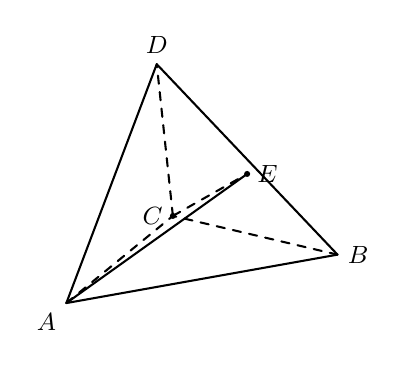
\begin{tikzpicture}[x=0.82cm,y=0.82cm,line cap=round,line join=round,line width=0.75pt,font=\small]
\coordinate (A) at (0,0);
\coordinate (B) at (4.2,0.75);
\coordinate (D) at (1.4,3.7);
\coordinate (C) at (1.65,1.35);
\coordinate (E) at (2.8,2.0);
\draw (A)--(B)--(D)--cycle;
\draw[dashed] (A)--(C)--(B);
\draw[dashed] (C)--(D);
\draw (A)--(E);
\draw[dashed] (C)--(E);
\fill (C) circle (1.1pt);
\fill (E) circle (1.1pt);
\node[below left] at (A) {$A$};
\node[right] at (B) {$B$};
\node[above] at (D) {$D$};
\node[left] at (C) {$C$};
\node[right] at (E) {$E$};
\end{tikzpicture}
\end{center}
\nopagebreak[4]
   （1） 证明：平面 \(ACD\perp\) 平面 \(ABC\)；

   （2） 过 \(AC\) 的平面交 \(BD\) 于点 \(E\)，若平面 \(AEC\) 把四面体 \(ABCD\) 分成体积相等的两部分，求二面角 \(D-AE-C\) 的余弦值。

\end{question}
\begin{question}
\gkti{20}在直角坐标系中 \(xOy\)，曲线 \(C:y^2=2x\)，过点 \((2,0)\) 的直线 \(l\) 交 \(C\) 于 \(A,B\) 两点，圆 \(M\) 是以线段 \(AB\) 为直径的圆。

   （1） 证明：坐标原点 \(O\) 在圆 \(M\) 上；

   （2） 设圆 \(M\) 过点 \(P(4,-2)\)，求直线 \(l\) 与圆 \(M\) 的方程。

\end{question}
\begin{question}
\gkti{21}已知函数 \(f(x)=x-1-a\ln x\)。

   （1） 若 \(f(x)\ge0\)，求 \(a\) 的值；

\Needspace{5\baselineskip}
   （2） 设 \(m\) 为整数，且对于任意正整数 \(n\)，
\nopagebreak[4]
\[
   \left(1+\frac12\right)\left(1+\frac1{2^2}\right)\cdots\left(1+\frac1{2^n}\right)<m,
\]
   求 \(m\) 的最小值。

\end{question}
\begin{question}
\gkti{22}在直角坐标系 \(xOy\) 中，直线 \(l_1\) 的参数方程为
\nopagebreak[4]
\[
\begin{cases}
x=2+t,\\
y=kt,
\end{cases}\qquad(t\text{ 为参数}),
\]
\Needspace{5\baselineskip}
直线 \(l_2\) 的参数方程为
\nopagebreak[4]
\[
\begin{cases}
x=-2+m,\\
y=\dfrac{m}{k},
\end{cases}\qquad(m\text{ 为参数}).
\]
设 \(l_1\) 与 \(l_2\) 的交点为 \(P\)，当 \(k\) 变化时，\(P\) 的轨迹为曲线 \(C\)。

   （1） 写出 \(C\) 的普通方程；

   （2） 以坐标原点为极点，\(x\) 轴正半轴为极轴建立极坐标系，设 \(l_3:\rho(\cos\theta+\sin\theta)-\sqrt2=0\)，\(M\) 为 \(l_3\) 与 \(C\) 的交点，求 \(M\) 的极径。

\end{question}
\begin{question}
\gkti{23}已知函数 \(f(x)=|x+1|-|x-2|\)。

   （1） 求不等式 \(f(x)\ge1\) 的解集；

   （2） 若不等式 \(f(x)\ge x^2-x+m\) 的解集非空，求 \(m\) 的取值范围。

\end{question}